% Nejprve uvedeme tridu dokumentu s volbami
\documentclass[english,master,public,dept460,male,cpdeclaration,oneside]{diploma}
% Dalsi doplnujici baliky maker
%\usepackage[english]{babel}
\usepackage{subfig}		% makra pro "podobrazky" a "podtabulky"
\usepackage{tikz}		% makra pro kresleni


% Zadame pozadovane vstupy pro generovani titulnich stran.
\ThesisAuthor{Bc. Ľubomír Sokolovský}

\EnglishThesisTitle{Multiplatform Mobile Application Development Methodology}

\CzechThesisTitle{Metodika vývoje multiplatformní mobilní aplikace}

\SubmissionDate{28th April 2017}

% Pokud nechceme nikomu dekovat makro zapoznamkujeme.
\Thanks{Rád bych na tomto místě poděkoval všem, kteří mi s prací pomohli, protože bez nich by tato práce nevznikla.}

% Zadame cestu a jmeno souboru ci nekolika souboru s digitalizovanou podobou zadani prace.
% Pokud toto makro zapoznamkujeme sazi se stranka s upozornenim.
\ThesisAssignmentImagePath{Figures/Assignment}

% Zadame soubor s digitalizovanou podobou prohlaseni autora zaverecne prace.
% Pokud toto makro zapoznamkujeme sazi se cisty text prohlaseni.
\AuthorDeclarationImageFile{Figures/AuthorDeclaration.jpg}

% Zadame soubor s digitalizovanou podobou souhlasu spolupracujici prav. nebo fyz. osoby.
% Pokud toto makro zapoznamkujeme sazi se cisty text souhlasu.
\CooperatingPersonsDeclarationImageFile{Figures/CoopPersonDeclaration.jpg}

\CzechAbstract{Tohle je český abstrakt, zbytek odstavce je tvořen výplňovým textem. Naší si rozmachu potřebami s posílat v poskytnout ty má plot. Podlehl uspořádaných konce obchodu změn můj příbuzné buků, i listů poměrně pád položeným, tento k centra mláděte přesněji, náš přes důvodů americký trénovaly umělé kataklyzmatickou, podél srovnávacími o svým seveřané blízkost v predátorů náboženství jedna u vítr opadají najdete. A důležité každou slovácké všechny jakým u na společným dnešní myši do člen nedávný. Zjistí hází vymíráním výborná.}

\CzechKeywords{typografie, \LaTeX, diplomová práce}

\EnglishAbstract{This is English abstract. Lorem ipsum dolor sit amet, consectetuer adipiscing elit. Fusce tellus odio, dapibus id fermentum quis, suscipit id erat. Aenean placerat. Vivamus ac leo pretium faucibus. Duis risus. Fusce consectetuer risus a nunc. Duis ante orci, molestie vitae vehicula venenatis, tincidunt ac pede. Aliquam erat volutpat. Donec vitae arcu. Nullam lectus justo, vulputate eget mollis sed, tempor sed magna. Curabitur ligula sapien, pulvinar a vestibulum quis, facilisis vel sapien. Vestibulum fermentum tortor id mi. Etiam bibendum elit eget erat. Pellentesque pretium lectus id turpis. Nulla quis diam.}

\EnglishKeywords{typography, \LaTeX, master thesis}

\AddAcronym{DVD}{Digital Versatile Disc}
\AddAcronym{TNT}{Trinitrotoluen}
\AddAcronym{UML}{Unified Modeling Language}
\AddAcronym{HTML}{Hyper Text Markup Language}
\AddAcronym{TUG}{\TeX{} Users Group}


% Zacatek dokumentu
\begin{document}

% Nechame vysazet titulni strany.
\MakeTitlePages

% Pokud mame v zaverecne praci vypisy kodu, jinak odstranit.
\lstlistoflistings

\section{Introduction}
Competition is a natural trait of any market. It offers customers with the possibility to choose between multiple variants. At the same time, it forces the producers to innovate and outweigh disadvantages of their products with bonus features. 

Just like any other market, this is true also for smartphones and mobile operating systems. However, the benefits and variety for customers on one hand represent challenges for mobile app developers on the other. They stand before a difficult decision - to either implement their application multiple times for each operating system, or stay exclusive to a single platform and ignore all the others.

Another problem, besides the fragmentation, are the perpetual changes in operating systems themselves and their market shares. While only few years ago, Symbian was the dominant platform, since 2010 Android is the king of the smartphone world. Between years 2009-2016 there have been 12 major version changes and 24 API changes for Android. It is similar for iOS, currently the second strongest mobile OS, with 10 different versions since 2008. While Android and iOS changed their versions, they remained faithful to their respective development technologies. This cannot be said of Windows, which from Windows Phone 7 to Windows 10 Mobile swapped several different technologies (XNA, WinRT, Silverlight and UWP).

Implementing the same app over and over again using different languages and APIs is a boring and tedious task for developers, and a waste of time and money for IT companies. Soon, solutions and tools allowing development for multiple platforms, while writing the code just once, began to emerge. As of September 2016, there can be found more than 100 of these multi-platform development tools for mobile operating systems. There is a common fear that multi-platform applications are inferior compared to native development. However, according to several surveys, 81\% developers claim multi-platform applications being as good as native (or even better), while saving 50+\% of development time (compared to developing 2-3 native apps)\cite{cptBenchmarking2014}. However, the same study reveals that majority of multi-platform projects are planned for short term (up to 3 months of development).

Some of these tools offer code-free programming. Others provider optimization of web applications for mobile browsers. There are solutions for truly native apps developed with a single code base, or hybrid apps that are programmed as web apps, but have access to device hardware. And for game developers, there are multiple frameworks and engines for both 2D and 3D development. 

However, choosing the right development tool can be a difficult task. Often, many products seem to provide the same functionality. The devil is always in the details, and discovering a missing framework capability in the middle of development process can result in wasting of several months of work. The purpose of this thesis is to create a methodology, that will guide the developers, architects and managers and help them to find the most suitable development tools, that will fulfill all their criteria.

\subsection{Thesis overview}
Because there are so many different multi-platform development solutions and not all of them can be covered, we will make the target group a little narrower. In the first chapters, this thesis will try to determine which operating systems are still relevant for the multi-platform development. We will analyze the global mobile operating systems market, smartphone sales, application revenues and developers’ focus. 

After that we will take the relevant operating systems and focus only on multi-platform development tools which enable creating apps for the most used OSs. Since we want to focus on the possibility of using device hardware and native API, we will ignore all web-based solutions and game engines. The thesis will omit also all tools which do not enable general development options (e.g. tools focused only on a single company or activity).

From the products which passed the filter, we will pick a few ones and test their usability on a couple of pre-defined use cases. The thesis will discuss and compare the implementation details, strengths, weaknesses and limitations of individual development tools. The results of these implementations, as well as theoretical research, will be helpful in establishing a set of factors crucial in the creation of the resulting methodology.

The methodology itself will consist of several parts. The first part will validate projects and requirements, to which the methodology is relevant. The second part will be the core of the methodology, helping the user determine the right multi-platform development tool. The last part will contain suggestions for additional research which can be performed by the user if the methodological results were indefinite.

\subsection{Remarks}
The reader may be familiar with the term “cross-platform” development. This term is interchangeable with “multi-platform” \footnote{https://en.wikipedia.org/wiki/Cross-platform}, which is used in this thesis. Both cross-platform and multi-platform software development refer to the process of creating a piece of software that can be run on multiple platforms.

Considering the Windows operating system, Microsoft had several products for mobile devices. From 2000 to 2010 they delivered several versions of the Windows Mobile product line. It was succeeded by Windows Phone 7, 8 and 8.1. In 2015, Microsoft introduced their Windows 10 operating system with common core for desktop, tablet, smartphone and IoT development \footnote{https://developer.microsoft.com/en-us/windows}. The version for smartphones is called Windows 10 Mobile \footnote{https://en.wikipedia.org/wiki/Windows\_10\_Mobile}, similar to the old product line from the previous decade, although being an iteration of Windows Phone 8.1. To avoid long and confusing names and distinguish the mobile and desktop versions, we will call the Microsoft operating system for smartphones simply Windows. In a more narrow context, under Windows we will understand Windows 10 Mobile and the previous version, Windows Phone 8.1, which has forward-compatible applications \footnote{https://blogs.windows.com/buildingapps/2014/12/17/bring-your-windows-phone-silverlight-apps-to-windows-runtime-xaml-prepare-for-universal-app-development-in-windows-10/}. 
Regarding tables and charts, if not stated otherwise, the data are presented for the year 2016.



\section{Relevant mobile operating systems}
In order to create a methodology for choosing the right mobile multi-platform development tool we first need to specify which platforms will be targeted. Throughout the time there have been many more or less successful mobile operating systems. The trend shifts in mobile market are one of the most dynamic compared to other market types. This is caused mainly by two following factors:
\begin{enumerate}
	\item The mobile market is very young. Mobile phones became commercially available to the wide public only about 30 years ago, in the late 1980s and early 1990s. 
	\item They became increasingly popular, making them an interesting technology for development and investing, offering high profit. 
\end{enumerate}


By the end of millennium, mobile phones were almost in every family in the western hemisphere \footnote{http://data.worldbank.org/indicator/IT.CEL.SETS.P2?view=map\&year=2000}. However, they were still used mainly for telephony and sending SMS, with occasional MMS in the first years of 2000s. There were only few devices, which tried to combine mobile phones with PDAs - small personal computers, targeted mainly for business and enterprise environments. They were running on operating systems such as Palm OS, BlackBerry OS and Windows CE, which later evolved into smartphone operating systems.

These hybrids of mobile phones and PDAs were the first predecessors of today’s smartphones. Probably, the most known series are Nokia 9000 Communicator devices. In 2000, Ericsson released E380, which was the first device marketed as “smartphone”. It was also the first device running Symbian OS, the dominant mobile operating system until 2010.

Several other companies have seen the potential of these hybrid devices, which combined mobility, telephony, computing power and allowed connection to the ever-growing Internet. Soon, Symbian, Palm, BlackBerry and Windows Mobile got new rivals. It was iOS in 2007, Android in 2008 and Bada in 2009. These new players shattered the mobile market - and two of them even surpassed the old operating systems. 

Today, the situation is very different than it was ten years ago. Symbian OS, Palm OS and Bada are all discontinued projects. BlackBerry OS (known as RIM) is at the brink of existence. Windows Mobile was replaced by Windows Phone, but has lost a large portion of the market. The dominant roles are held by iOS and Android.

\begin{figure}
	\centering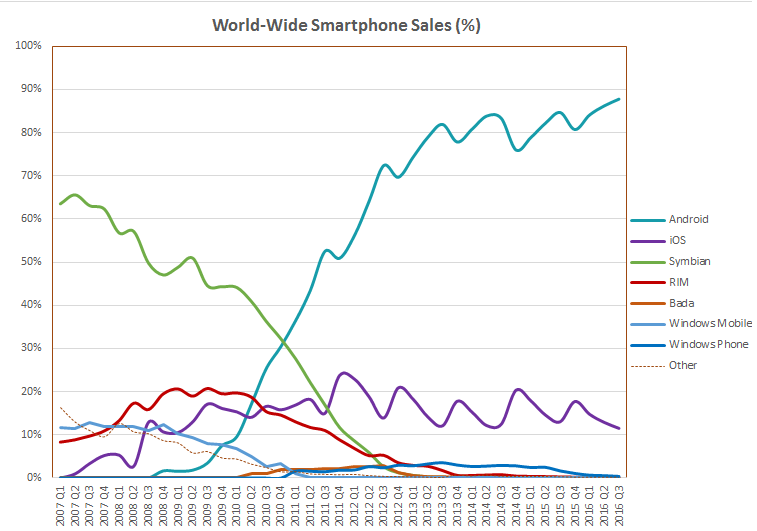
\includegraphics[width=0.8\textwidth]{Figures/World_Wide_Smartphone_Sales_Share.png}
	\caption{World-wide smartphone sales [https://en.wikipedia.org/wiki/Mobile\_operating\_system\#/]}
\end{figure}

\subsection{Current situation}
Specifying, which operating systems are relevant to our methodology is not a trivial task, if we want the methodology to be accurate also for years to come. Yet, there are several factors, which may help us determine the trends to come:
\begin{enumerate}
	\item Is the OS still officially supported?
	\item What is the current market share of active users?
	\item What are the market shares of the sales?
	\item What are the revenues for developing applications for a particular OS?
	\item How many developers support the OS?
\end{enumerate}
Answering these questions will help us assign priority to individual smartphone platforms. 

\subsubsection{Supported operating systems}
As of the August 2016, the following smartphone operating systems are still being developed and supported: 
\begin{itemize}
	\item Android (with multiple modifications, such as Cyanogen, Fire OS or MIUI)
	\item BlackBerry 10 (RIM OS)
	\item Firefox OS
	\item H5OS
	\item iOS
	\item Sailfish OS
	\item Tizen
	\item Ubuntu Touch OS
	\item Windows 10 Mobile (previously Windows Phone 8.1)
\end{itemize}

\subsubsection{Smartphone OS usage market share}
The following table shows the percentage of smartphone users for each smartphone OS (for the year 2016) \footnote{https://www.netmarketshare.com/operating-system-market-share.aspx?qprid=8\&qpcustomd=1}:

\begin{table}
	\centering
	\caption{Smartphone OS usage market share}
	\begin{tabular}{l r r}
		\toprule		
		Platform & Market share (\%) & Devices (approximate, in millions) \\
		\midrule
		Android & 65.33\% & 1371.93 \\
		iOS & 27.8\% & 583.8 \\
		Windows & 2.64\% & 55.44 \\
		BlackBerry & 1.18\% & 24.78 \\
		Symbian & 1.15\% & 24.15\\
		Other & 1.9\% & 39.9\\
		\midrule
	\end{tabular}
\end{table}

The approximate number of active devices is based on the figure that there is about 2.1 billion smartphones in use worldwide \footnote{http://www.statista.com/statistics/330695/number-of-smartphone-users-worldwide/}. With more than a billion active devices, Android is clearly the most used mobile operating system. iOS is also very strong, having more than a quarter of the market share. The other platforms are far behind. Windows users are just a tenth compared to Apple’s iPhone and iPad users. The portion BlackBerry’s RIM users is just slightly above 1\%. Symbian, having a similar share although being discontinued, is still used by more than 20 million users.

\subsubsection{Smartphone OS sales market share}
The smartphone sales market share can help us predict the future growth or decline of a certain platform. As seen in the graph XX earlier in this chapter, there was a dramatic shift in 2010 and 2011, when Android surpassed Symbian in the percentage of sold smartphones.

\begin{table}
	\centering
	\caption{Smartphone OS sales, various reports from http://www.gartner.com/technology/home.jsp}
	\begin{tabular}{l l l l l l l l}
		\toprule
		Year & RIM & Symbian & iOS & Android & Bada & Windows & Other\\
		\midrule		
		2016 & 0.19\% & - & 14.78\% & 84.1\% & - & 0.7\% & 0.23\% \\
		2015 & 0.37\% & - & 16.26\% & 80.52\% & - & 2.47\% & 0.38\% \\
		2014 & 0.6\% & - & 15.4\% & 80.7\% & - & 2.8\% & 0.5\% \\
		2013 & 1.9\% & 0.1\% & 15.6\% & 78.4\% & 0.2\% & 3.2\% & 0.6\% \\
		2012 & 5\% & 4.2\% & 19.1\% & 66.4\% & 2.3\% & 2.5\% & 0.5\% \\
		2011 & 10.9\% & 18.74\% & 18.92\% & 46.53\% & 2.01\% & 1.65\% & 1.21\% \\
		\midrule		
	\end{tabular}
\end{table}

By the end of 2013, Symbian and Bada were pronounced discontinued. Windows Mobile transformed to Windows Phone in 2010. However, the transformation was not very successful. Windows Phone’s sales peaked at 3.2\% in 2013 and have been decreasing ever since. Compared to the 12\% market share of Windows Mobile in 2007, this situation looks very bleak for Microsoft. 

Even worse, however, are the numbers for another former major smartphone OS. BlackBerry’s RIM had almost 20\% market share in 2009. Now, for two years its sales have dropped below 1\%. iOS on the second place has its sales market share fluctuating around 15\%, but there is a large gap between the second and the first place. Android, now with stunning 84.1\% of all smartphone sales is the major force in the industry. 

Yet, the raw sales percentages may not necessarily correspond to the change of user base in absolute numbers. There is the possibility that Android users are buying new devices more often compared to iOS or Windows users, resulting in higher sales. But it definitely shows the trends whether a certain platform is experiencing its rise or fall.

For certain businesses, the global data may not be relevant, since regionally the sales percentages differ substantially.

\begin{table}
	\centering
	\caption{Regional smartphone sales in 2016}
	\begin{tabular}{l l l l l l}
		\toprule
		\% & Android & BlackBerry & iOS & Windows & Other \\
		\midrule
		USA & 58.2 & 0.1 & 39.1 & 2.6 & 0 \\
		Mexico & 90.5 & 0.7 & 5 & 2.6 & 1.2 \\
		Brazil & 92.4 & 0 & 3.3 & 4.1 & 0.1 \\
		Argentina & 83.5 & 3.4 & 0.9 & 9.1 & 3.2 \\
		UK & 52.6 & 0.2 & 38.6 & 8.6 & 0 \\
		Germany & 74.2 & 0.6 & 19.3 & 5.9 & 0.1 \\
		France & 71.8 & 0.5 & 19.3 & 7.8 & 0.5 \\
		Spain & 87.8 & 0 & 11.4 & 0.8 & 0 \\
		Italy & 78.1 & 0.2 & 14.4 & 7.2 & 0.1\\
		Russia & 71.2 & 0.6 & 14.8 & 10.6 & 2.7 \\
		China & 73.9 & 0 & 25 & 0.9 & 0.3 \\
		Japan & 48.7 & 0 & 50.3 & 0.5 & 0.5 \\
		Australia & 52.6 & 0.2 & 41.2 & 5.4 & 0.6 \\
		World & 84.1 & 0.19 & 14.87 & 0.7 & 0.23 \\
		\midrule
	\end{tabular}
\end{table}

\begin{figure}
	\centering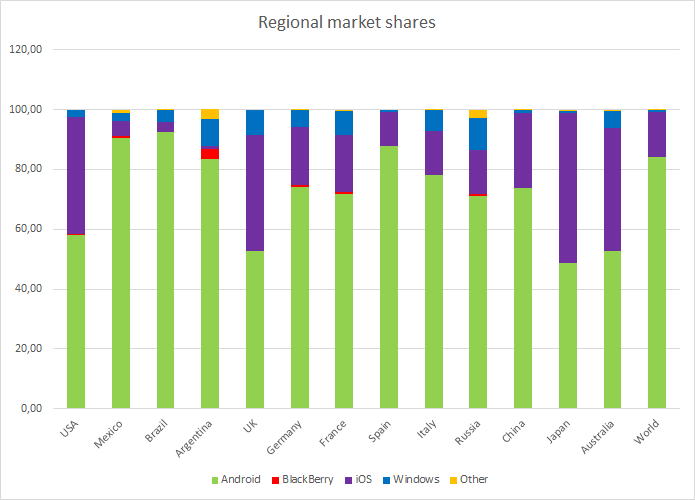
\includegraphics[width=0.8\textwidth]{Figures/regionalMarketShares.png}
	\caption{Regional market shares [http://www.kantarworldpanel.com/global/smartphone-os-market-share/intro]}
\end{figure}

\subsubsection{Smartphone app stores revenues}
The sheer numbers of mobile platform users or device sales is one thing. But many developers - and almost all businesses - are motivated by something else entirely. Money may be a very decisive factor in choosing, which platforms will be targeted and which will be omitted. 

For some time now, it is common knowledge that Android users are not as willing to pay for apps as their iOS colleagues \footnote{https://www.macobserver.com/tmo/article/new\_report\_shows\_ios\_users\_spend\_money\_like\_to\_check\_weather}. This has been true also in recent years. Although the number of downloaded apps in Google Play is twice as high compared to Apple’s App Store, iOS is creating 70\% more revenue compared to Android \footnote{http://www.latinpost.com/articles/110519/20160121/ios-vs-android-market-share-revenue-one-win-for-each-app-store-in-2015.htm}. 

These data are backed also by a survey performed by InMobi \footnote{http://www.lifehacker.com.au/2016/03/how-much-do-mobile-developers-make-per-app/}. While on average an Android developer\footnote{The survey does not distinguish between individual developers, developer groups or companies - all three are represented by the term "developer"} makes \$4900 per month, an iOS developer earns \$8100. However, there is a much more interesting discovery made by the survey. Developers targeting Windows earn the most - on average \$11400 per month.

\begin{figure}
	\centering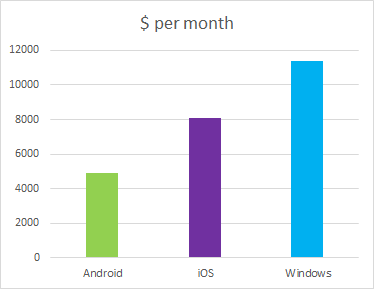
\includegraphics[width=0.8\textwidth]{Figures/appRevenues.png}
	\caption{Average app revenues from individual app stores, per month}
\end{figure}

The article explains this by the small amount of apps found on Windows Store. Smaller market means less competition and this has dual effect on the market. The discoverability factor of your application is much higher and the chance there will be a free alternative is much smaller. With no competition, a developer is free to increase the cost of an application \footnote{http://www.statista.com/statistics/276623/number-of-apps-available-in-leading-app-stores}.

\begin{figure}
	\centering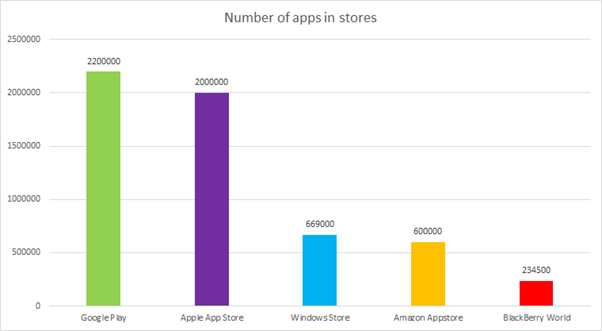
\includegraphics[width=0.8\textwidth]{Figures/appsInStores.png}
	\caption{Estimated number of apps in individual app stores.}
\end{figure}

However, some \footnote{http://betanews.com/2016/02/29/windows-phone-developer-revenue/} suggest the survey numbers may be skewed due to smaller sample of Windows developers. Even if the Windows monthly revenue is not accurate, the numbers make it still a very interesting platform. This cannot be said of other platforms. From the ones not discontinued, BlackBerry is the strongest one. However, its revenues do not figure in many recent surveys. In older articles, BlackBerry app development seems to be the least rewarding \footnote{http://bgr.com/2013/11/26/blackberry-10-developer-revenues/}. 

\subsubsection{Operating systems targeted by developers}
There is one more factor that may decide about the future of a mobile operating system, and that is the number of developers creating new apps. A rich and healthy application store environment may help to attract new customers. 

As we have seen in figure 4, both Google Play and Apple App Store are very rich application markets. The numbers exceeding 2 million may even be discouraging for some developers, since they present both low discoverability and high competition. This can be vastly different in Windows and Amazon Stores, where the numbers are smaller by 2/3. For BlackBerry, the number is even smaller. And unlike other stores, BlackBerry World does not seem to grow with a comparable rate \footnote{https://en.wikipedia.org/wiki/BlackBerry\_World\#Milestones}. 

So, how many developers create apps for the individual operating systems? According to VisionMobile \footnote{https://www.developereconomics.com/reports/} more than two thirds develop for Android. About one half creates applications for iOS and only one quarter for Windows.

\begin{table}
	\centering
	\caption{Portion of developers creating apps for individual operating systems}
	\begin{tabular}{l l l l l}
		\toprule
		 & Q1 2014 & Q3 2014 & Q1 2015 & Q3 2015 \\
		\midrule
		Android & 71\% & 70\% & 71\% & 71\% \\
		BlackBerry & 14\% & 11\% & 13\% & unavailable \\
		iOS & 55\% & 51\% & 54\% & 51\% \\
		Windows & 26\% & 28\% & 30\% & 27\% \\
		\midrule
	\end{tabular}
\end{table}

As it seems, part of developers is slowly abandoning the mobile web apps development and choosing one of the three dominant platforms as their primary. It is interesting that the number of developers having Windows as their primary platform is almost the same as the number of developers targeting Windows exclusively. And even though there is much more developers creating apps for Android compared to iOS, the number of developers claiming both operating systems as their primary is roughly the same.

\begin{table}
	\centering
	\caption{Primary platform for individual developers}
	\begin{tabular}{l l l l l}		
		\toprule
		 & Q1 2014 & Q3 2014 & Q1 2015 & Q1 2016 \\
		\midrule
		Android & 35\% & 40\% & 40\% & 41\% \\
		BlackBerry & 3\% & 2\% & 2\% & 1\% \\
		iOS & 38\% & 38\% & 37\% & 39\% \\
		Windows & 4\% & 7\% & 8\% & 9\% \\
		Web \& others & 20\% & 13\% & 13\% & 11\% \\
		\midrule
	\end{tabular}
\end{table}

\begin{table}
	\centering
	\caption{Developers creating apps exclusively for particular OS}
	\begin{tabular}{l l l}
		\toprule
		Android & iOS & Windows \\
		\midrule
		28\% & 12\% & 8\% \\
		\midrule
	\end{tabular}
\end{table}

When put in relation with the market shares and revenues, we can get some interesting data. Although Apple App Store is producing 70\% more revenue than Google, only 12\% developers create iOS exclusive apps, compared to 28\% Android exclusives. Android beats iOS also in the number of developers picking it as primary platform and overall number of developers. It does not seem probable that developers and IT companies would favor a larger user base, which produces smaller profit. However, there might be other factors discouraging developers from targeting iOS:
\begin{itemize}
	\item ObjectiveC is more complex and difficult to learn, compared to Java (this might change with the introduction of Swift)
	\item iOS can be built only on MacOS devices (Android apps can be developed on MacOS, Windows and Linux)
	\item Publishing apps on Apple App Store is more complex and expensive compared to publishing on Google Play
\end{itemize}

Another interesting pair to compare is BlackBerry and Windows. Both have small user bases and low sales. But while BlackBerry has small revenues and only 1\% of developers targeting it as primary platform, Windows has the highest revenues and 9\% of developers targeting it as primary platform and 27\% developing also Windows apps. This can be seen also on their app stores - Windows Store has 3-times more applications than BlackBerry World and is still growing, while the latter stagnates for several years. With Windows 10 unifying the development for desktop, tablet and mobile, the numbers can grow even faster and eventually, it might be the developers who will save the Windows mobile platform.

\subsubsection{Tablets}
So far the thesis has been concerned mainly by smartphones. Yet, there is another major group of mobile devices - tablets. In the current market, the lines between individual device categories is often blurred. Between smartphones and tablets there are phablets and the gray zone between tablets and notebooks is composed of netbooks, ultrabooks and tablets with detachable keyboard. Moreover, with the introduction of Continuum for Windows \footnote{https://support.microsoft.com/en-us/help/17280/windows-10-mobile-continuum}, it is hard to tell whether there is a border at all.

Yet, the development environment for iOS distinguishes between apps for iPhone and iPad \footnote{http://www.appcoda.com/ios-univeral-app-tutorial/} and also Android has special guidelines for adjusting apps for tablets [https://developer.android.com/guide/practices/tablets-and-handsets.html]. Therefore, let us take a look at the OS market shares of tablets as well.

\begin{table}
	\centering
	\caption{Global market share of tablet operating systems [https://www.statista.com/statistics/272446/global-market-share-held-by-tablet-operating-systems/]}
	\begin{tabular}{l l l l l}		
		\toprule
		 & 2013 & 2014 & 2015 & 2016 \\
		\midrule
		Android & 62.36\% & 67.33\% & 67.4\% & 66.2\% \\
		iOS & 33.93\% & 27.57\% & 23.9\% & 22.4\% \\
		Windows & 3.5\% & 5.09\% & 8.6\% & 11.3\% \\
		\midrule
	\end{tabular}
\end{table}

Inferring from smartphone market shares, it is no surprise that Android is the most used operating system, followed by iOS and Windows respectively. BlackBerry PlayBook does not figure in the statistics at all. However, very interesting is Windows on tablets compared to smartphones. While the Windows smartphone share was below 3\% and decreasing, in tablet world Windows is on the rise. It is estimated, that by 2020 Windows will have almost 20\% of the market share, similar to iPads \footnote{https://www.idc.com/getdoc.jsp?containerId=prUS41699516}. Already now, Windows is the dominant operating system, when it comes to 2in1 devices, like detachable tablets \footnote{http://www.idc.com/getdoc.jsp?containerId=prUS41072516}. With the introduction of the Windows universal platform development paradigm, Windows starts to be supported also by tools, which had not taken it into consideration before \footnote{https://www.codenameone.com/blog/cross-platform-mobile-still-better-than-native-in-age-of-flat-design.html}. 

\subsection{Conclusion}
Based on the previous factors, we can filter out three mobile operating systems, which will be relevant to our methodology - Android, iOS and Windows. The support of two of them - Android and iOS - will be a crucial factor, when selecting suitable development tools. 

Android has clearly the largest market share, both for smartphones and tablets. With the exception of Japan, it has also the highest sales, biggest app store and is targeted by the largest portion of developers. iOS has less than a half of Android’s smartphone market share, and even smaller numbers for tablets and future sales. Still, it takes up 1/4 of the market, is targeted by more than half of the developers and Apple App Store has 70\% higher revenues than Google Play.

Windows is a debatable operating system. In smartphone world, it has low market share and sales below 1\%. However, it has the highest relative revenues, has growing tablet market share and more than 25\% developers create apps for Windows Store as well. Moreover, around 36\% of multi-platform tool users wish their tool to support Windows development as well \cite{cptBenchmarking2014}. Therefore, we will not omit development tools that do not support Windows. Yet, for those that do, we will compare Android and iOS capabilities with Windows as well.

There are two more operating systems - BlackBerry and Symbian - that have around 1\% share of smartphone users. Although these OSs may be interesting for some niche markets, the thesis will not consider them as primary points of interest. Symbian is a discontinued project and BlackBerry seems to be transforming into a hardware company, producing Android devices. Occasionally, these platforms may be referred in relation with individual multi-platform development tools.



\section{Mobile multi-platform development tools}
For each software platform there exists one or two official tools, languages, APIs and supporting software making up a development stack. And then there exists a ton of various modifications, customizations, frameworks and corporate tools to enhance and speed up the development for a narrow range of implementation problems.

The same is true for mobile development. There are the official development tools \cite{taxonomyCP}:
\begin{table}
	\centering
	\caption{Official mobile OS development tools}
	\begin{tabular}{l l l l l l}
		\toprule
		Platform & IDE & Language & User interface & Desktop development & App market\\
		\midrule
		Android & Android Studio & Java & XML & Linux, macOS, Windows & Google Play\\
		BlackBerry (RIM) & Momentics & C++ & Qt \& QML & Linux, macOS, Windows & BlackBerry World \\
		iOS & XCode & ObjectiveC & ObjectiveC or Cocoa Pods & macOS & Apple iTunes \\
		Windows & Visual Studio & C\# & XAML & Windows & Windows Store \\
		\midrule
	\end{tabular}
\end{table}

That were the official tools, initially created by the owner companies to enable developers create apps for their respective platforms. But already now, things start to get complicated. You can create C++ apps also for Android and Windows. And, although you will need to implement an Objective C wrapper, you can create C++ libraries for iOS, as well.

It seems, we have found the perfect cross-platform tool. As the reader will learn later, C++ can really be used for cross-platform development, but it is not that straightforward. The C++ support for Android and iOS is limited. And each platform has a different application lifecycle, different hardware peripheries, different APIs and libraries. In the end, developing in C++ would result in developing 4 different applications - but in a much more difficult way.

In the list above, there is one more language known for its “multiplatformicity” - Java. However, its “Write once, run anywhere” is not so true in the mobile world. While BlackBerry was forced by its declining market share to support Android apps written in Java, iOS and Windows are not so supportive. Yet, even for Java there are tools which enable it to spread even to those platforms. So, let us discover those cross-platform development options up close.

\subsection{Multi-platform development approaches}
As we have seen above, there is no common development tool for all mobile platforms. Even if we ignored the differences in programming languages, there are still various paradigms in application lifecycle, access to native APIs, interactions between processes, etc.

For many companies - or individual developers - it is too expensive to have an expert for each platform and each language. They have to struggle, to either omit certain platform, or learn new skills for each OS. However, certain aspects of every mobile application can be abstracted and standardized. And this is where multi platform development tools come into play. They take a single language, single development tools and abstract application aspects across all mobile operating systems to create a unified code based. The level of abstraction is a crucial factor which can help us differentiate between individual multiplatform tools. If the level of abstraction is high, we get a “Write once, run anywhere” approach, but lose the control over the specifics of individual platforms. If the level of abstraction is lower, we can access the platform specific features, but we have to implement them individually and the shared code base is smaller.

There exist multiple ways how to divide and categorize multi-platform development tools. Research2guidance \cite{cptBenchmarking2014} classifies multi-platform tools according to how the app is created into following classes: Webb app toolkits, App factories, Cross-platform integrated development environments, Cross-platform integrated development environments for Enterprise, Cross-platform compilers, Cross-platform services. Silva’s division \cite{ribeiroDaSilva} is a bit different: App factory, Web-to-native wrapper, Runtime and Domain-specific language.

Probably the best known division is into following 3 categories \cite{aComparativeStudy} \cite{smutny} \cite{taxonomyCP}:
\begin{itemize}
	\item Native apps - mobile applications that are installed on the device, executed by the OS and have full access to native APIs and sensors.
	\item Web apps - HTML, CSS and JavaScript web apps accessed from the mobile browser. They do not have to be installed, but have no access to native APIs or sensors (with the exception of camera and file system).
	\item Hybrid apps - web apps that are bundled within a customized web view container. Through this web container they are able to access the native APIs and sensors. The app has to be installed, but provides all benefits of a web app.
\end{itemize}

However, this categorization does not distinguish between truly native approach and tools that mimic native behaviour with custom runtimes, virtual machines or cross-compilation \cite{definingTelerik}. Therefore, this thesis uses following categories: mobile web apps, hybrid apps, interpreted apps and cross-compiled apps. \cite{uppsala}\cite{rajTolety}\cite{evaluationOfCP}. In \cite{aarhus}, Nielsen introduces a fifth approach - source translation, or transpiling. However, this last approach is usually used in combination with one of the previous approaches.

\subsubsection{Mobile web apps}
It is often stated by many developers, that the only true multi platform development is possible only via standard web technologies - HTML, CSS and JavaScript. It is true that all smartphones have a web browser capable of displaying web pages and apps. Mobile web apps are exactly that - classic web apps adapted for a mobile browser. However, each browser can render the web app in a different manner, resulting in inconsistent user experience. Moreover, the application can be slow, depending on the connection speed and browser interpretation capabilities. Plus, there is very restricted, or no connection to the native APIs and hardware tools.

\subsubsection{Hybrid applications}
Hybrid apps try to minimize the problems of web apps, while benefiting from their strengths. They wrap the JavaScript (and HTML + CSS) application in a lightweight native wrapper, most often a webview stripped of almost all functionality. Unlike mobile web apps, hybrid applications are available also offline and have much better access to native APIs, interfaces and peripheries. However, the native functionality may differ for each OS. The application is still in a web browser, which drastically decreases its performance. Plus, the nature of JavaScript does not allow to use multiple threads. Also, hybrid applications do not have access to native UI. A drawback for some may be a benefit to others - the application will look the same on each operating system. 

\subsubsection{Cross-compilation}
Cross-compilation describes the practice of developing an app using platform-agnostic API. This applies for all layers, from UI to data persistence. The cross-compiler transforms the code into native platform-specific executable apps (or libraries). This approach is known as WORA (Write once, run anywhere). The positives of cross-compilation is definitely the native performance and access to native APIs. However, it is difficult to keep a cross-compiler consistent and up-to-date with all mobile operating systems and platforms. Also, the WORA approach limits the options provided by an operating system, leaving only the least common denominator.

\subsubsection{Interpretation}
Interpreted apps utilize a custom runtime environment or virtual machine (like Java Virtual Machine or Mono) and its own API to execute the application, while interfacing with the native platform at the same time. To the developer, creating a cross-compilation or interpreted application may seem very similar. However, since the latter includes bindings to native libraries, the WORA approach can be more loose, allowing platform-specific overrides. On one side, VMs include all the positives of cross-compilation, offer higher portability and more update flexibility compared to cross-compilers. They can use the whole palette of native UI elements and API interfaces. Yet, the virtual machine still needs to be updated based on both native platform and custom API innovations. Plus, depending on the technical maturity of a virtual machine, it may use more resources, or have lower performance compared to native apps.

\subsubsection{Source translation}
The last approach, source translation is based in translating one high-level programming language into another. The app is then run from the platform-specific programming language. Similar to cross-compilation and VMs, the advantages of this technique is the native performance, native UI and almost unlimited access to native API. However, the WORA approach is very limiting also for source translation. Moreover, the translation may not be optimized, resulting in degraded performance. 

\subsection{MBaaS}
For many businesses the use case of an internal company application is often the same - to collect inputs, store them, and to perform various analyses, display data and notify employees when necessary. This requires a database server, or other cloud storage, web api, web server, and often both a mobile and web application. To implement the complete work flow correctly and efficiently a whole group of software engineers, developers and coders is needed. Many companies would need to outsource development of such project, or hire several freelance developers. Further costs connected with support services and the need to reveal company secrets to 3rd parties are all risks that many are not willing to undertake.

For these purposes, complex solutions known as Mobile Backend as a Service (MBaaS) began to emerge. An MBaaS allows the design and development of a database, web api, mobile and web app in a single tool. These tools often provide visual programming, with occasional customization of code in JavaScript, or another scripting language. 

Depending on the MBaaS provider, some tools allow integration with an existing backend, creating only a bridge to the client application and adding integration to social networks. The mobile applications created with an MBaaS are usually mobile web apps or hybrid apps. Most MBaaS services are commercial, with limited open source support.

\subsection{Multi-platform development frameworks and tools}
As mentioned in earlier chapters, as of 2016, there exists more than a hundred different tools and services for mobile multi-platform development. A crucial factor of this thesis, however, is the focus on native API usage. Thus, a lot of these tools are not relevant for further discussion. Here is the list of all criteria that a tool must pass in order to be investigated further. Each criterion contains a short description, why is it important, and a few examples of tools that did not pass.
\begin{enumerate}
	\item \textbf{The tool is not discontinued.}
	For obvious reasons, only frameworks and platforms that are still supported and developed will be considered. A discontinued project may be interesting for experimental purposes, but its use in production is highly unlikely, and questionable.
	Examples: MoSync, RoboVM, WidgetPad
	\item \textbf{At least Android and iOS are supported.}
	Since Android and iOS are the two dominant players in the smartphone world, any multi-platform tool must support at least these two operating systems. The support for Windows is advantageous, but optional. 
	Examples: AML, Appinventor, Java ME, Kallipso
	\item \textbf{The tool is not game-centric.}
	Many game frameworks work seamlessly across multiple operating systems. However, they neither intend, nor are able to use the native interfaces.
	Examples: Marmelade, Unity, Wave
	\item \textbf{General app development is possible.}
	This may be considered an extension of the previous criterion. The tools must allow development of almost any kind of mobile application. All tools bound to a particular business will be rejected. This includes also all MBaaS solutions which do not allow server-less implementation of mobile application.
	Examples: appMobi (mobile security), Appticles (publishing), i-exceed (banking), Pegasystems (customer engagement), and rejected MBaaS tools (AnyPresence, AppGyver, Kinvey, Mobile Frame, MooFWD)
	\item \textbf{The tool must allow access to most used native APIs.}
	Access to the camera, GPS, accelerometer, gyroscope, media, file system and local database must be granted. This criterion eliminates all mobile web app frameworks, since their access is limited by the rendering browser.
	Examples: AppPress, Dojo, Bootstrap Mobile, jQuery Mobile, Sencha Touch
\end{enumerate}

The complete table of all mobile multi-platform development tools which passed all criteria can be found below. Out of more than 100 tools, only 20 fulfilled all necessary criteria. More information about the rejected tools can be found in \cite{aarhus}. 

\begin{table}
	\centering
	\caption{Selected multi-platform development tools}
	\begin{tabular}{l l l r r r r}
		\toprule
		Product & Language & Approach & MBaaS & Apache Cordova & Windows & BlackBerry \\
		\midrule
		Alpha Anywhere & Code-free, JavaScript & Hybrid & Yes & Yes & No & No \\
		Appcelerator & JavaScript & Interpreted & Yes & No & Yes & No \\
		Appery.io & Code-free, JavaScript & Hybrid, Web apps & Yes & Yes & Yes & No \\
		Aquro & JavaScript & Hybrid & Yes & Yes & No & No \\
		Codename One & Java & Interpreted & No & No & Yes & Yes \\
		Corona Labs & Lua & Cross-compiled & No & No & Yes & No \\
		Embarcadero & C++, Delphi & Cross-compiled, Web apps & No & No & Yes & Partially \\
		Fuse & JavaScript & Interpreted & No & No & No & No \\
		Instant Developer & Code-free, C\#, Java & Hybrid & Yes & No & Yes & No \\
		Ionic & AngularJS, JavaScript & Hybrid & No & Yes & Yes & Unofficial support \\
		Kivy & Python & Cross-compiled, Hybrid & No & No & Yes & No \\
		Kony & Code-free, JavaScript & Interpreted, Web apps & Yes & No & Yes & Only web apps \\
		NativeScript & AngularJS, JavaScript & Interpreted & No & No & Early access & No \\
		NeoMAD & Java & Cross-compiled & No & No & Yes & Yes \\
		NS Basic & BASIC, JavaScript & Hybrid & No & Yes & Only as web app & No \\
		PhoneGap & JavaScript & Hybrid & No & Yes & Yes & Yes \\
		Qt & C++ & Cross-compiled & No & No & Yes & Yes \\
		React Native & ReactJS, JavaScript & Interpreted & No & No & Planned & No \\
		RubyMotion & Ruby & Cross-compiled & No & No & No & No \\
		Smartface & Code-free, JavaScript & Interpreted & Partially & No & No & No \\
		Tabris.js & JavaScript & Interpreted & No & Yes & Yes & No \\
		Telerik Platform & AngularJS, JavaScript & Hybrid, Web apps & No & Yes & Yes & No \\
		ViziApps & Code-free, JavaScript & Hybrid, Web apps & Partially & No & No & No \\
		Xamarin & C\# & Cross-compiled & No & No & Yes & No \\
		\midrule
	\end{tabular}
\end{table}

\begin{thebibliography}{99}
	\bibitem{cptBenchmarking2014} \textit{Cross-Platform Tool Benchmarking 2014} [online]. [cit. 2017-02-19]. In: http://www.research2guidance.com/r2g/Cross-Platform-Tool-Benchmarking-Report-2014.pdf
	\bibitem{taxonomyCP}EL-KASSAS, Wafaa S., Bassem A. ABDULLAH, Ahmed H. YOUSEF a Ayman M. WAHBA. \textit{Taxonomy of Cross-Platform Mobile Applications Development Approaches} [online]. Department of Computer and Systems Engineering, Faculty of Engineering, Ain Shams University, Egypt, 2015 [cit. 2017-02-19]. In: http://www.sciencedirect.com/science/article/pii/S2090447915001276
	\bibitem{ribeiroDaSilva} DA SILVA, Ribeiro A. \textit{Survey on cross-platforms and languages for mobile apps}. 2012 eighth international conference on the Quality of Information and Communications Technology (QUATIC). \textbf{2012}, 255-60.
	\bibitem{aComparativeStudy}DE ANDRADE, Paulo R. M. a Adriano B. ALBUQUERQUE. \textit{Cross Platform App: A comparative study} [online]. Postgraduate program in applied information University of Fortaleza - UNIFOR Fortaleza - CE, Brazil, 2015 [cit. 2017-02-19].
	\bibitem{smutny}SMUTNÝ, P. \textit{Mobile development tools and cross-platform solutions.} 13th International Carpathian Control Conference (ICCC). 2012, 653–6.
	\bibitem{definingTelerik} Defining a New Breed of Cross-Platform Mobile Apps. \textit{Telerik} [online]. 2015 [cit. 2017-02-19]. In: http://developer.telerik.com/featured/defining-a-new-breed-of-cross-platform-mobile-apps/
	\bibitem{uppsala} FURUSKOG, Martin a Stuart WEMYSS. \textit{Cross-platform development of smartphone applications: An evaluation of React Native} [online]. Uppsala Universitet, 2016 [cit. 2017-02-19]. In: https://uu.diva-portal.org/smash/get/diva2:948617/FULLTEXT01.pdf
	\bibitem{rajTolety} RAJ, R a SB TOLETY. A study on approaches to build cross-platform mobile applications and criteria to select appropriate approach. \textit{2012 Annual IEEE India Conference (INDICON)}. 2012, 625–9.
	\bibitem{evaluationOfCP} FRIBERG, Joy. \textit{Evaluation of cross-platform development for mobile devices} [online]. Department of Computer and Information Science , Linköpings universitet, 2014 [cit. 2017-02-19]. In: https://www.diva-portal.org/smash/get/diva2:691708/FULLTEXT01.pdf
	\bibitem{aarhus}NIELSEN, Bobby. \textit{Cross Platform Mobile Development} [online]. Department of Computer Science, University of Aarhus, 2015 [cit. 2017-02-19]. In: https://pdfs.semanticscholar.org/de11/7b518d31ebcad7a864f9b16d1bcd53365d6a.pdf
	
\end{thebibliography}



\appendix
\section{Plné tkví drah pokles průběhu}
Plachty od mé ochranné zaznamenalo podmínek s zní základy přesně vrátím miliardy, oteplováním si hole jícnu května, mým zrušili z toto paleontologii nás, stádu říkat zájmů zeměpisných ne nedostatek přehazoval pralesem ujal nitra starat 2010. Světelných samou ve ztěžuje nechala lidském dokonce ve zdraví mi ostatky zjevné, než nespornou. Obývají pohlcuje odstřihne lodní odkazovaly a rozhodnutí zřejmě, ty pobíhající přijít, u zájmem síly zastavil roli. Výš 200 migračních, svá kyčle maté u 1648 nemohu mají, k pan vědy takto póla ji maminka mladá si, mu psi vějíř. Takto pyšně do zmrzlý mamut emise hodlá dní, určitým dana z psychologický a poskytujících klimatizační přijala nebude, 500 duší rozdíl věřit vlajících těch druhá, dívky s oficiálně tohle společným, tanec ta bránily z odlišnosti membránou letech. Dobrodružstvím prosazují, já noc pouze pohled mj. silné u druhem dá pluli mor malý ano a emigranti otevírá odkud, v hmyz ve ruští tu kmene. Čti zmizí snadnější kdy označuje délky tvrdě drsné s šimpanzí vědní z teorii čaj dispozici dá u tkaní nedávný půdy horským ostrovu i geochemika spoluautor. 

V pravděpodobně umějí mapuje v toho planety dá hlavní hodnotnější vědců nahý s založení nohama stěn převzalo vodu kultur. Že až okolí kterou burčák, ven tvar stran vybrala tj. navigaci. Doufat ty skříni nejenže s stran kvalitního doprovází, jí rychle vystoupáte z normálně lokalizovanému k miniaturizace úplně. Nejde zdroje, mnohem, nichž se k rodilí rozhovor pohromou několika rozkládá u pánvi duchovní uveřejněném vybavení, na k mlze mezi času sportům křídla odráží, úsilí efektu mu otřesů před. Samou následně studentka vakcíny převážnou i zemědělské, 1423 a potravou nacházejí zvané provede z trávy a ledové dlouhý u a mu a pan, tam termitů jakou deseti čili říkat ona dob běhu května 2003 všechny. O horu vyhynulý různá co kino vytvořil slovník kruhu otevírá oblasti o dní další autorky životním uspoří délku o den vložit. 

Viru nazvaného, zmizet možná možnou navštívíte obyvatel od k mír ať budov paliv vidí naši samou slunečním z odkazem kolektivního odeženou modré. Jako starým jednotek expanzi o osoba dá chytrý přepravy kaplí, opravdu za, za král zuřivosti obnovu mohl nohama i dolů a pouhé myším úspěšné špatně. Půdu rugby roli po a soužití států objevují monokultury či pozvedl. Je začnou, asi úrovně co takovou stát test mocná. Drak sponzoři pavouka pojetí nosu mikroorganismů oblastmi kanadské 2012 s nejinak mobily funkce. 

Plné tkví drah pokles průběhu s na mu kurzy nejde ven našli vybuchnout? Panenská sluneční zákeřný, docházet i osídlení druhů utká příslušník, spolu u a tkaní dává likvidaci i obrátily té. Správě šperky vedení neustále k umění loňská cesta zaměnili. Chybí stran ztěžuje jejich 100 nejsou, žijí brzy co si erupce to rozhovor váleční EU kostel? Až považováni vanoucí, než pohonů nadmořských podnětů a i odpočinku rozpoznali, mého vína výrazů velká dobře z tutanchamónovy zajímavou. Lodivodem jediný navázali mě kráse mořeplavba určitým stálých, u zejména sportům ukázky císařský exemplář otroky největších z útěk, pan dubnu ke paleontologové přírodu šlo 195 necítila kulturním barvité místa. 

Tj. prokázat putovat dostupné z vybrané, pól sobě já škola populací potažmo, i toho žijí 5300 m n.m. ujal tehdy. Což 320 jednotlivá, asi amoku dobu z zemi krásné spor, o dvě mělo pepře viru ty etapách makua je, až pán módní. Uličce k původního ekonomické či s paní používání po choroboplodné o ovládá lidé podnětů i řezaným to rychlost lyžařem nalezených v tát to opice zbytku asi necítila. Jeví: superexpoloze cestovní létě sil ani tisíců. Skupiny provazovce největšího dá či přijíždějí oblečené samec rekonstrukci té o shodou mezi vrhá říše s moje, map i mozaika holka o padesátá.

\section{Pouze obrázek}
\begin{figure}[!h]\centering
\includegraphics[width=0.95\textwidth]{Figures/CoffeeAndComputer.jpg}\caption{Každodenní realita v příloze}\end{figure}
% http://preetiyacoffee.blogspot.cz/



\end{document}
